\newpage
\subsubsection{Module opération}
\begin{figure}[h!]  
  \centering
    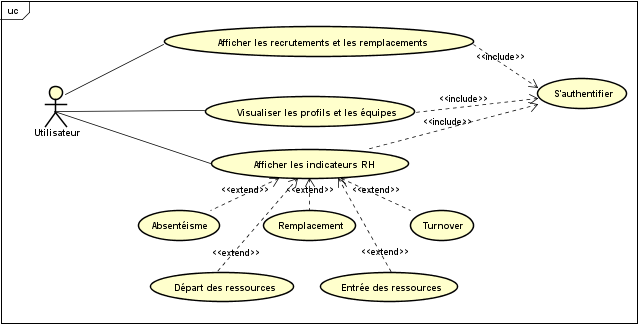
\includegraphics[width=0.95\textwidth]{chapitre2/Figures/ressourcesUC.png}
  \caption{Diagramme de cas d’utilisation du module de suivi des ressources}
\end{figure}
\subsubsection*{Description des cas d’utilisations }
\begin{itemize}[label=\textbullet]

%Afficher les groupes des TPE
\item \textbf{Afficher les groupes des TPE :}
\begin{table}[!h]
\begin{tabular}{|p{15cm}|}%p{2.5cm}|p{9cm}
\rowcolor{shadecolor}\multicolumn{1}{|c|}{Sommaire d’indentification} \\
\hline
\textbf{objectif : } cette fonctionnalité permet d'fficher les groupes des TPE\\
\textbf{acteurs : } utilisateur\\
\textbf{précondition : } 
	\begin{itemize}[label=\textbullet]
	\item l'acteur est connecté au système
	\item l'acteur a le droit d'accès
	\end{itemize}
	\\
\hline
\rowcolor{shadecolor}\multicolumn{1}{|c|}{Description des scénarios} \\
\hline
	\textbf{Scénario nominal :}
	\begin{itemize}[label=\textbullet]
	\item scénario "Afficher les groupe des TPE" :
		\begin{itemize}
		\item l'acteur demande de visualiser l'ensemble des groupes des TPE
		\item le système affiche un tableau contenant l'ensemble des groupes des TPE.
		\end{itemize}
	\end{itemize}
	\\
\hline
\end{tabular}
\centering \caption{Description du cas d’utilisation "Afficher les groupes des TPE"} \label{TablePR}
\end{table}

\newpage
%Visulaliser tous les TPE par groupe
\item \textbf{Visulaliser la liste des TPE par goupe :}
\begin{table}[!h]
\begin{tabular}{|p{15cm}|}%p{2.5cm}|p{9cm}
\rowcolor{shadecolor}\multicolumn{1}{|c|}{Sommaire d’indentification} \\
\hline
\textbf{objectif : } cette fonctionnalité permet de visualiser la liste des TPE affiché par groupe\\
\textbf{acteurs : } utilisateur\\
\textbf{précondition : } 
	\begin{itemize}[label=\textbullet]
	\item l'acteur est connecté au système
	\item l'acteur a le droit d'accès
	\end{itemize}
	\\
\hline
\rowcolor{shadecolor}\multicolumn{1}{|c|}{Description des scénarios} \\
\hline
	\textbf{Scénario nominal :}
	\begin{itemize}[label=\textbullet]
	\item scénario "Visulaliser la liste des TPE" :
		\begin{itemize}
		\item le système affiche l'ensemble des TPE regroupés par groupes
		\end{itemize}
	\end{itemize}
	\\
\hline
\end{tabular}
\centering \caption{Description du cas d’utilisation "visualiser la liste des TPE affiché par groupe"} \label{TablePR}
\end{table}

%Afficher les TPE d'un seule groupe
\item \textbf{Afficher les TPE d'un groupe :}
\begin{table}[!h]
\begin{tabular}{|p{15cm}|}%p{2.5cm}|p{9cm}
\rowcolor{shadecolor}\multicolumn{1}{|c|}{Sommaire d’indentification} \\
\hline
\textbf{objectif : } cette fonctionnalité permet d'afficher la liste des TPE d'un groupe\\
\textbf{acteurs : } utilisateur\\
\textbf{précondition : } 
	\begin{itemize}[label=\textbullet]
	\item l'acteur est connecté au système
	\item l'acteur a le droit d'accès
	\end{itemize}
	\\
\hline
\rowcolor{shadecolor}\multicolumn{1}{|c|}{Description des scénarios} \\
\hline
	\textbf{Scénario nominal :}
	\begin{itemize}[label=\textbullet]
	\item scénario "Afficher les TPE d'un groupe" :
		\begin{itemize}
		\item le système affiche l'ensemble des TPE du groupe
	
		\end{itemize}
	\end{itemize}
	\\
\hline
\end{tabular}
\centering \caption{Description du cas d’utilisation "Afficher les TPE d'un groupe"} \label{TablePR}
\end{table}

%Chercher un groupe des TPE 
\newpage
\item \textbf{Chercher un groupe des TPE :}
\begin{table}[!h]
\begin{tabular}{|p{15cm}|}%p{2.5cm}|p{9cm}
\rowcolor{shadecolor}\multicolumn{1}{|c|}{Sommaire d’indentification} \\
\hline
\textbf{objectif : } cette fonctionnalité permet de chercher un groupe des TPE \\
\textbf{acteurs : } utilisateur\\
\textbf{précondition : } 
	\begin{itemize}[label=\textbullet]
	\item l'acteur est connecté au système
	\item l'acteur a le droit d'accès
	\end{itemize}
	\\
\hline
\rowcolor{shadecolor}\multicolumn{1}{|c|}{Description des scénarios} \\
\hline
	\textbf{Scénario nominal :}
	\begin{itemize}[label=\textbullet]
	\item scénario "Chercher un groupe des TPE" :
		\begin{itemize}
		\item l'acteur saisie les critères de recherche dans dans les champs de saisie
		\item le système filtre les données selon : code du groupe, nom du banque
		\item le système affiche le groupe cherché
	
		\end{itemize}
	\end{itemize}
	\\
\hline
\end{tabular}
\centering \caption{Description du cas d’utilisation "Chercher un groupe des TPE"} \label{TablePR}
\end{table}

%Chercher un TPE 
\item \textbf{Chercher un TPE :}
\begin{table}[!h]
\begin{tabular}{|p{15cm}|}%p{2.5cm}|p{9cm}
\rowcolor{shadecolor}\multicolumn{1}{|c|}{Sommaire d’indentification} \\
\hline
\textbf{objectif : } cette fonctionnalité permet de chercher un TPE \\
\textbf{acteurs : } utilisateur\\
\textbf{précondition : } 
	\begin{itemize}[label=\textbullet]
	\item l'acteur est connecté au système
	\item l'acteur a le droit d'accès
	\end{itemize}
	\\
\hline
\rowcolor{shadecolor}\multicolumn{1}{|c|}{Description des scénarios} \\
\hline
	\textbf{Scénario nominal :}
	\begin{itemize}[label=\textbullet]
	\item scénario "Chercher un TPE" :
		\begin{itemize}
		\item l'acteur saisie les critères de recherche dans dans les champs de saisie
		\item le système filtre les données selon : code du TPE, code du groupe, nom du banque
		\item le système affiche le TPE cherché
	
		\end{itemize}
	\end{itemize}
	\\
\hline
\end{tabular}
\centering \caption{Description du cas d’utilisation "Chercher un TPE"} \label{TablePR}
\end{table}

%Configurer les informations demandées 
\item \textbf{Configurer les informations demandées du TPE :}
\begin{table}[!h]
\begin{tabular}{|p{15cm}|}%p{2.5cm}|p{9cm}
\rowcolor{shadecolor}\multicolumn{1}{|c|}{Sommaire d’indentification} \\
\hline
\textbf{objectif : } cette fonctionnalité permet l'acteur de demander l'ensemble des informations du TPE \\
\textbf{acteurs : } utilisateur\\
\textbf{précondition : } 
	\begin{itemize}[label=\textbullet]
	\item l'acteur est connecté au système
	\item l'acteur a le droit d'accès
	\end{itemize}
	\\
\hline
\rowcolor{shadecolor}\multicolumn{1}{|c|}{Description des scénarios} \\
\hline
	\textbf{Scénario nominal :}
	\begin{itemize}[label=\textbullet]
	\item scénario "Configurer les informations demandées du TPE" :
		\begin{itemize}
		\item l'acteur précise les informations demandées du TPE
		\item le système filtre enregistre l'ensemble des informations demandées.
	
		\end{itemize}
	\end{itemize}
	\\
\hline
\end{tabular}
\centering \caption{Description du cas d’utilisation "Configurer les informations demandées du TPE"} \label{TablePR}
\end{table}




\end{itemize}